\section{Experiments}

%The main motivation for this work is the potential to train \dgp models in an efficient and scalable manner without compromising on predictive performance and retain accurate quantification of uncertainty.
%In view of these criteria, 
We  evaluate our model by comparing it against relevant alternatives for both regression and classification, and assess its performance when applied to large-scale datasets.
We also investigate the extent to which such deep compositions continue to yield good performance when the number of layers is significantly increased.
%% An asynchronous distributed version of the model is also discussed in the supplementary material.

\subsection{Model Comparison}

\input{figures/comparison_2l.tex}

We primarily compare our model to the state-of-the-art \dgp inference method presented in the literature, namely \dgp{s} using expectation propagation~\citep[\dgpep;][]{Bui16}.
We originally intended to include results for the variational auto-encoded \dgp~\citep{Damianou13}; however, the results obtained using the available code were not competitive with \dgpep and we thus decided to exclude them from the figures.
We also omitted \dgp training using sequential inference~\citep{Wang16} given that we could not find an implementation of the method and, in any case, the performance reported in the paper is inferior to more recent approaches.
% Although the main goal of this paper is to develop a \dgp technique which improves over the state-of-the-art, 
We also compare against \dnn{s} in order to present the results in a wider context, and demonstrate that \dgp{s} lead to better quantification of uncertainty.
Finally, to substantiate the benefits of using a deep model, we  compare against the shallow sparse variational \gp~\cite{HensmanMG15} implemented in GPflow~\cite{GPflow2016}.

We use the same experimental set-up for both regression and classification tasks using datasets from the UCI repository~\citep{Asuncion07}, for models having one hidden layer.
The results for architectures with two hidden layers are included in the supplementary material.
The specific configurations for each model are detailed below:
\begin{description}[style=unboxed,leftmargin=0.1cm]
\item[\dgprbf, \dgparc]: In the proposed \dgp with an \rbf kernel, we use $100$ random features at every hidden layer to construct a multivariate GP with $D_F^{(l)}=3$, and set the batch size to $m=200$.
%% Given that lower precision is required in the initial phase of the optimization procedure, 
We initially only use a single Monte Carlo sample, and halfway through the allocated optimization time, this is then increased to $100$ samples.
We employ the Adam optimizer with a learning rate of $0.01$, and in order to stabilize the optimization procedure, we fix the parameters $\Thetavect$ for $12,000$ iterations, before jointly optimizing all parameters.
As discussed in Section~3.3, $\Omegavect$ are optimized variationally with fixed randomness.
The same set-up is used for \dgparc, the variation of our model implementing the \arccosine kernel;
%
\item[\textsc{dgp-ep}]\footnote{Code obtained from: \\ \url{github.com/thangbui/deepGP_approxEP}}: 
For this technique, we use the same architecture and optimizer as for \dgprbf and \dgparc, a batch size of $200$ and $100$ inducing points at each hidden layer. %, and we also set the dimensionality of \gp{s} at the hidden layers to $3$.
%% The Adam optimizer is initialized in an identical manner.
For the classification case, we use $100$ samples for approximating the Softmax likelihood;
%\item[\textsc{dgp-var}]\footnote{Code obtained from: \\ \url{github.com/zhenwendai/DeepGP/tree/master/deepgp}}: As above, $100$ inducing points and a dimensionality of $3$ is employed at every hidden layer.
%For the multi-layer perceptron in the recognition model, we use the provided standard settings.
%Feed-forwarding of the original inputs is disabled;
%\item[\textsc{dgp}]\footnotemark[\value{footnote}]: The set-up of this model is identical to that of \dgpvar, with the exception that the recognition model is absent;
\item[\textsc{dnn}]: We construct a \dnn configured with a dropout rate of $0.5$ at each hidden layer in order to provide regularization during training.
In order to preserve a degree of fairness, we set the number of hidden units in such a way as to ensure that the number of weights to be optimized match those in the \dgprbf and \dgparc models when the random features are taken to be fixed. 
\end{description}

We assess the performance of each model % by running the optimization procedure and periodically evaluate 
using the error rate (\rmse in the regression case) and mean negative log-likelihood (\mnll) on withheld test data.
The results are averaged over $3$ folds for every dataset.
The experiments were launched on single nodes of a cluster of Intel Xeon E5-2630 CPUs having $32$ cores and $128$GB RAM.
% while ensuring that the runs for all methods are allocated a fair amount of resources.
 
Figure~\ref{fig:error_vs_time} shows that \dgprbf and \dgparc consistently outperform competing techniques both in terms of convergence speed and  predictive accuracy.
This is particularly significant for larger datasets where other techniques take considerably longer to converge to a reasonable error rate, although \dgpep converges to  superior \mnll for the \protein dataset.
The results are also competitive (and sometimes superior) to those obtained by the variational \gp (\vargp) in \citet{HensmanMG15}. 
It is striking to see how inferior uncertainty quantification provided by the \dnn (which is inherently limited to the classification case, so no \mnll reported on regression datasets) is compared to \dgp{s}, despite the error rate being comparable. % and a substantial degree of overfitting can be observed.
% \notePM{We don't need the acronym \dgpvar as we don't show results here.} 
% --> EB commented out above as I think \dgpvar was wrong, I replaced it with \vargp
 
By virtue of its higher dimensionality, larger configurations were used for \mnist.
For \dgprbf and \dgparc, we use $500$ random features, $50$ \gp{s} in the hidden layers, batch size of $1000$, and Adam with a $0.001$ learning rate. % , and fix $\thetavect$ for $12,000$ iterations.
Similarly for \dgpep, we use $500$ inducing points, with the only difference being a slightly smaller batch size to cater for issues with memory requirements.
Following~\citet{Simard03}, we employ $800$ hidden units at each layer of the \dnn.
The \dgprbf peaks at $98.04\%$ and $97.93\%$ for $1$ and $2$ hidden layers respectively.
It was observed that the model performance degrades noticeably when more than $2$ hidden layers are used (without feeding forward the inputs).
This is in line with what is reported in the literature on \dnn{s}~\citep{Neal96,Duvenaud14}.
By simply re-introducing the original inputs in the hidden layer, the accuracy improves to $98.2\%$ for the one hidden layer case. % \noteEB{???, problem was with deeper settings, no?}.

Recent experiments on \mnist using a variational \gp with \mcmc report overall accuracy of $98.04\%$~\cite{Hensman15}, while the \autogp architecture has been shown to give $98.45\%$ accuracy~\cite{Krauth17}.
Using a finer-tuned configuration, \dnn{s} were also shown to obtain $98.5\%$ accuracy~\cite{Simard03}, whereas $98.6\%$ has been reported for \svm{s}~\cite{Scholkopf97}.
In view of this wider scope of inference techniques, it can be confirmed that the results obtained using the proposed architecture are comparable to the state-of-the-art, even if further extensions may be required for obtaining a proper edge.
Note that this comparison focuses on approaches without preprocessing, and excludes convolutional neural nets.

%As highlighted in the introduction to this work, one of the distinctive features of \dgp{s} is the ability to quantify the uncertainty of predictions. 
%Matching the results presented in Figure~\ref{fig:error_vs_time}, a complete comparison of the \mnll obtained by these models is presented in the supplementary material, where it is noted that the rate of progression of this metric is consistent with the results for error rate.

%\begin{table}[h]
%\caption{Comparison of accuracy for the proposed \dgprbf approach with previous results on \mnist. The comparison focuses on approaches without preprocessing, and excludes convolutional neural nets.} \label{tab:results:MNIST}
%\label{tab:results:mnist} 
%\begin{center}
%\begin{tabular}{lc}
%{\bf ALGORITHM}   & {\bf ACC.} \\
%\hline \\
%Sparse GP-LVM       \citep{Gal14}  & $94.00\%$ \\
%GP Hashing     \citep{Ozdemir16} &  $\sim 95.00\%$ \\
%MCMC VAR-GP      \citep{Hensman15}  & $98.04\%$ \\
%DNN			\citep{Simard03}		  	   & $98.50\%$    \\
%SVM          \citep{Scholkopf97}           & $98.60\%$ \\
%DGP-RFF 0HL                & $98.36\%$ \\
%DGP-RFF 1HL                & $98.10\%$ \\
%DGP-RFF 2HL                & $97.44\%$ \\
%\end{tabular}
%\end{center}
%\end{table}

\subsection{Large-scale Datasets}

One of the defining characteristics of our model is the ability to scale up to large datasets without compromising on performance and accuracy in quantifying uncertainty.
As a demonstrative example, we evaluate our model on two large-scale problems which go beyond the scale of datasets to which \gp{s} and especially \dgp{s} are typically applied.

\begin{table}[t]
\caption{{Performance of our proposal on large-scale datasets.}}\label{tab:results:LARGE}
\label{tab:results:large} 
\begin{center}
\begin{tabular}{lcc}
{\bf Dataset}   & 
\begin{tabular}{c}
{\bf Accuracy} \\
\begin{tabular}{cc}
\rbf & \arc
\end{tabular}
\end{tabular} & \begin{tabular}{c}
{\bf MNLL} \\
\begin{tabular}{cc}
\rbf & \arc
\end{tabular}
\end{tabular}\\
\hline \\
\mnisteight    & \begin{tabular}{cc} $99.14\%$ & $99.04\%$  \end{tabular} & \begin{tabular}{cc} $0.0454$ & $0.0465$  \end{tabular}\\
\airline     &\begin{tabular}{cc} $78.55\%$ & $72.76\%$ \end{tabular} & \begin{tabular}{cc} $0.4583$ & $0.5335$  \end{tabular}\\
\hline
\end{tabular}
\end{center}
\end{table}

We first consider \mnisteight, which artificially extends the original \mnist dataset to $8+$ million observations.
We trained this model using the same configuration described for standard \mnist, and we obtained $99.14\%$ accuracy on the test set using one hidden layer. 
Given the size of this dataset, there are only few reported results for other \gp models.
Most notably, \citet{Krauth17} recently obtained $99.11\%$ accuracy with the \autogp framework, which is comparable to the result obtained by our model.

Meanwhile, the \airline dataset contains flight information for $5+$ million flights in the US between Jan and Apr 2008.
Following the procedure described in~\citet{Hensman13} and~\citet{Wilson16}, we use this $8$-dimensional dataset for classification, where the task is to determine whether a flight has been delayed or not.
We construct the test set using the scripts provided in~\citet{Wilson16}, where $100,000$ data points are held-out for testing.
%% Given the lower dimensionality of this dataset (8 features), 
We construct our \dgp models using $100$ random features at each layer, and set the dimensionality to $D_{F^{(l)}} = 3$. 
As shown in Table~\ref{tab:results:large}, our model works significantly better when the \rbf kernel is employed. 
In addition, the results are also directly comparable to those obtained by~\citet{Wilson16}, which reports accuracy and $\mnll$ of $78.1\%$ and $0.457$, respectively. 
These results give further credence to the tractability, scalability, and robustness of our model.

\subsection{Model Depth}
%
%In view of the existing literature on \dgp{s}, as well as the findings presented in~\citet{Duvenaud14}, the models discussed insofar have been limited to few hidden layers.
In this final part of the experiments, we assess the scalability of our model with respect to additional hidden layers in the constructed model.
In particular, we re-consider the \airline dataset and evaluate the performance of \dgprbf models constructed using up to $30$ layers. 
In order to cater for the increased depth in the model, we feed-forward the original input to each hidden layer, as suggested in~\citet{Duvenaud14}.

\input{figures/depth_experiment}

Figure~\ref{fig:depth} reports the progression of error rate and \mnll over time for different number of hidden layers, using the results obtained in~\citet{Wilson16} as a baseline (reportedly obtained in about $3$ hours).
As expected, the model takes longer to train as the number of layers increases.
However, the model converges to an optimal state in every case in less than a couple of hours, with an improvement being noted in the case of $10$ and $20$ layers over the shallower $2$-layer model.
The box plot within the same figure indicates that the negative lower bound is a suitable objective function for carrying out model selection.
%% Finally, we note that the baselines were reportedly obtained after about $3$ hours, whereas our models converge in less time. \notePM{Can we be more positive: it is worth noting that convergence times are also in favor of our approach, which decreases by $x \%$ in our experiments.}


%\subsection{Distributed Implementation}
%\noteKC{Will be moved to the supplementary material. Should be replaced with a short experiment on `very' deep DGPs.}
%Our model is easily amenable to a distributed implementation using asynchronous distributed stochastic gradient descent \citep{Chilimbi14, MartinAbadi15}. Our distributed setting\footnote{Currently, we use a CPU-only compute cluster.}, based on TensorFlow, includes one or more \emph{Parameter servers} (PS), and a number of \emph{Workers}. 
%The latter proceed asynchronously using randomly selected batches of data: they fetch fresh model parameters from the PS, compute the gradients of the loss function with respect to these parameters, and push those gradients back to the PS, which update the model accordingly. 
%Given that workers compute gradients and send updates to PS asynchronously, the  discrepancy between the model used to compute gradients and the model actually updated can degrade training quality. 
%This is exacerbated by a large number of asynchronous workers, as noted in \cite{Chen16}.
%
%We focus our experiments on the MNIST dataset, and study how training time and error rates evolve with the number of workers introduced in our system. 
%The parameters for the model are identical to those reported for the previous experiment.
%
%\pgfplotsset{label style={font=\Large}, title style={font=\Large}}
%\pgfplotsset{label style={font=\Large}, title style={font=\Large}}

\begin{figure}[ht]
\begin{center}
%% \begin{tabular}{c}
 {\scriptsize \bf  MNIST} \\
%% {\small MNIST-8M}\\
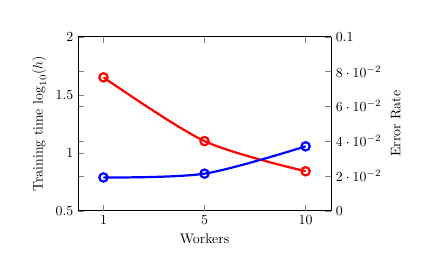
\begin{tikzpicture}[scale=0.5]
\begin{axis}[
    xmin=0, xmax=4,
  axis y line*=left,
	width=8cm, height=6cm,
  ylabel={Training time $\log_{10}(h)$},
  ymin=0.5, ymax=2,
  xlabel=Workers,
  xmin = 0.75, xmax = 3.25,
  xtick= {1,2,3},
  xticklabels={},
  extra x ticks={1,2,3},
  extra x tick style={xticklabels={1,5,10}}
  %xticklabels={0,1,5,10,15},
]
\addplot[smooth, mark=o, mark size=3pt, red, ultra thick]
coordinates{
    (1,1.65)
    (2,1.10)
    (3,0.84)
}; \label{plot_one}
%\addlegendentry{plot 1}
\end{axis}

\begin{axis}[
	width=8cm, height=6cm,
  ylabel={Error Rate},
  axis x line=none,
  xmin = 0.75, xmax = 3.25,
  ymin=0, ymax=0.1,
  ylabel near ticks, yticklabel pos=right
%% axis y line*=right
]
\addplot[smooth, mark=o, mark size=3pt, blue, ultra thick]
  coordinates{
    (1,0.0191)
    (2,0.0213)
    (3,0.037)
}; \label{plot_two}
%\addlegendimage{/pgfplots/refstyle=plot_one}\addlegendentry{plot 1}
%\addlegendimage{/pgfplots/refstyle=plot_two}\addlegendentry{plot 2}
\end{axis} 
\end{tikzpicture} 
%% &
%% \begin{tikzpicture}[scale=0.32]
%% \pgfplotsset{
%%     scale only axis,
%%     xmin=0, xmax=4
%% }

%% \begin{axis}[
%%   axis y line*=left,
%%   ylabel={Training time},
%%   ymin=6, ymax=17,
%%   xlabel=Workers,
%%   xmin = 0.75, xmax = 3.25,
%%   xtick= {1,2,3},
%%   xticklabels={},
%%   extra x ticks={1,2,3},
%%   extra x tick style={xticklabels={1,5,10}}
%%   %xticklabels={0,1,5,10,15},
%% ]
%% \addplot[smooth, mark=o, mark size=3pt, red, ultra thick]
%%   coordinates{
%%     (1,16)
%%     (2,12.6)
%%     (3,8)
%% }; \label{plot_one}
%% %\addlegendentry{plot 1}
%% \end{axis}

%% \begin{axis}[
%%   axis y line*=right,
%%   ylabel={Error Rate},
%%   axis x line=none,
%%   xmin = 0.75, xmax = 3.25,
%%   ymin=0, ymax=0.22
%% ]
%% \addplot[smooth, mark=o, mark size=3pt, blue, ultra thick]
%%   coordinates{
%%     (1,0.01)
%%     (2,0.04)
%%     (3,0.15)
%% }; \label{plot_two}
%% %\addlegendimage{/pgfplots/refstyle=plot_one}\addlegendentry{plot 1}
%% %\addlegendimage{/pgfplots/refstyle=plot_two}\addlegendentry{plot 2}
%% \end{axis} 
%% \end{tikzpicture}\\
%% \multicolumn{1}{c}{
\includegraphics[width=150pt]{figures/legend_async.pdf}
%% }
%% \end{tabular}
\end{center}
\caption{Comparison of training time and error rate for asynchronous \name{dgp-rbf} with 1, 5 and 10 workers.}
\label{fig:async}
\end{figure}

%
%We report the results in Figure~\ref{fig:async}, and as expected, the training time decreases in proportion to the number of workers, albeit sub-linearly.
%On the other hand, the increasing error rate confirms our intuition that imprecise updates of the gradients negatively impact the optimization procedure. 
%The work in \cite{Chen16} corroborates our findings.


%% \section{REMARKS}

%% \noteMF{
%% I believe we should have comparisons showing how well we do compared to alternative approaches to learn DGPs. 
%% If we show that we can learn better representations with less passes through the data compared to, say, inducing point formulations etc... I think we have some compelling evidence that what we propose is valuable; the fact that the idea is strightforward could even be used as way to say that we can do well with a simple approximation of DGPs as DNNs.
%% I think we should include results along these lines:
%% \begin{itemize}
%% \item Consider large-scale regression and classification problems
%% \item Show performance vs number of passes through the data (running time might not be reliable) 
%%   \begin{itemize}
%%   \item versus other DGP learning approaches where we can compare based on test likelihood and error rate (e.g., Expectation Propagation (Bui et al.), variational with inducing points (Hensman), variational GP (Ranganath and Blei), etc...)
%%   \item versus DNNs with other activations where we can compare based on error rate only (e.g., ReLU, sigmoid, etc...)
%%   \end{itemize}
%% \item What about showing results on autoencoders?
%% \item Scalability is sort of implied by the mini-batch formulation. Do we want to show performance wrt mini-batch size?
%% \item Anything else?
%% \end{itemize}
%% }
